\newpage
\section{Ricerca euristica}
La ricerca esaustiva non è praticabile in problemi di complesità esponenziale (e.g. $10^120$ configurazioni in scacchi). Noi usiamo
conoscenza del problemi es esperienza per riconoscere i cammini più promettenti, usiamo una stima del costo futuro, evitando di generare gli altri.
La conoscenza euristica (dal greco "eureka") aiuta fare scelte "oculate", questa ovviamente però non evita la ricerca ma la riduce, consente in
genere di trovare una buona soluzione in tempi accettabilili sotto certe condizioni garantisce completezza e ottimalità.\\\\
La conoscenza del problema data tramite una funzione di valutazione $f$, che include $h$ detta \textbf{funzione di valutazione euristica}.
$$h: n \to R$$
La funzione si applica al nodo ma dipende solo dallo stato (n.Stato).
\begin{note}
    Manteniamo la notazione in $n$ per unifomritò con $g$; $g$ dipende anche dal cammino fino al nodo.
\end{note}
$$f(n) = g(n) + h(n) \text{ove g(n) è il costo cammino visto con UC}$$
Per procedere preferibilmente verso il percorso migliore, seguendo problem-specific information, di stima del costo futuro:
\begin{itemize}
    \item La città più vicina (o la città più vicina alla metà in linea d'aria - tabella esterna) nel problema dell'itinerario.
    \item Il numero della caselle fuori posto nel gioco dell'otto.
    \item Il vataggio in pezzi della dama o negli scacchi
\end{itemize}

\begin{example}
    Mappa Romania dist. in linea d'aria.
    \begin{figure}[h!]
        \centering
        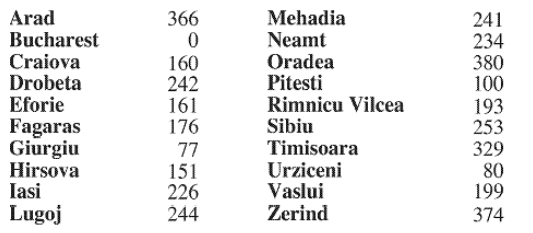
\includegraphics[width=0.75\textwidth]{images/esempio-euristica-h.png}
    \end{figure}
\end{example}

\subsection{Algoritmo di ricerca Best-first}
Il \textbf{best first - heuristic} usa lo stesso algoritmo di UC \footnote{Warning: AIMA ed. IV ha usato uno schema di
UC diverso e alcune proprietà cambiano} ma con uso di $f$ (stima di costo) per la coda con priorità.
Una volta scelta $f$ determina la strategia di ricerca. A ogni passo si sceglie il nodo sulla frontiera per cui il valore della $f$ è 
migliore (il nodo più promettente).
\begin{note}
    Migliore significa "minore" in caso di un'euristica che stima la distanza della soluzione
\end{note}
\hspace{-15pt}Un caso speciale: \textbf{greedy best-first}, su usa solo $h (f=h)$.
\begin{example}
    Esempio di greedy best-first con $f=h$
    \begin{figure}[h!]
        \centering
        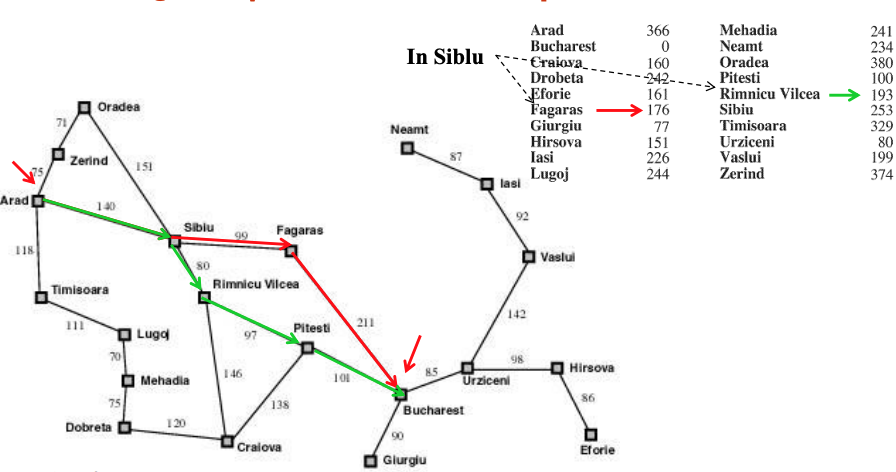
\includegraphics[width=0.75\textwidth]{images/esempio-best-first.png}
    \end{figure}
    Da Arad a Bucarest con \textbf{Greedy best-first}: Arad, sibiu, fagaras, bucharest (450) ma non è l'ottimale
    che sarebbe: Arad, Sibiu, Rimnicu, Pitesti, Bucarest (418).
\end{example}

\subsection{Algoritmo A}
Si può dire qualcosa di $f$ per avere garanzie di completezza e ottmialità?
\begin{definition}
    Un \textbf{Algoritmo A} è un algoritmo di best first con una fuzine di valutazione dello stato del tipo:
    $$f(n) = g(n) + h(n) \:\: \text{con}\:\: h(n) \geq 0 \:\: \text{e}\:\: h(goal) = 0$$
\end{definition}
In questa definizione abbiamo che $g(n)$ è il costo del cammino percorso per raggiugnere n, mentre $h(n)$ una
stima del costo per raggiungere da n un nodo goal (distanza).\\
Vedremo alcuni casi particolari dell'algoritmo A:
\begin{itemize}
    \item Se $h(n) = 0 [f(n) = g(n)]$ si ha \textbf{Ricerca Uniforme (UC)}.
    \item Se $g(n) = 0 [f(n) = h(n)]$ si ha \textbf{Greedy Best First}.
\end{itemize}
\begin{example}
    Esempio nel gioco dell'otto.
    \begin{figure}[h!]
        \centering
        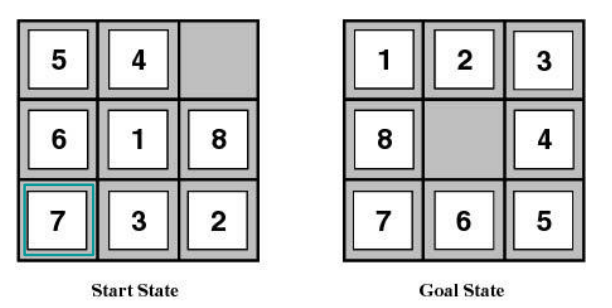
\includegraphics[width=0.6\textwidth]{images/esempio-gioco-otto.png}
    \end{figure}

    \hspace{-15pt}$f(n) = \#\text{mosse fatte} \:\: + \:\: \#\text{caselle-fuori-posto} \hspace{10pt} f(start) = 0 + 7 \hspace{10pt} f(goal-state) = ? + 0$\\
    Dopo $\leftarrow, \downarrow, \uparrow, \rightarrow$ abbiamo che $f = 4 + 7$, stesso stato, $g$ è cambiato.
\end{example}
\begin{theorem}
    L'algoritmo A con la condizione:
    $$g(n) \geq d(n) \cdot \epsilon \hspace{10pt}(\epsilon >0 \text{ costo minimo arco})$$
    è completo.
\end{theorem}
\begin{note}
    La conzione ci garantisce che non si verifichino situazioni strane del tipo:
    \begin{figure}[h!]
        \centering
        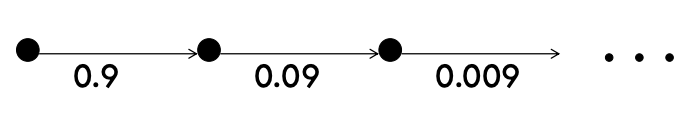
\includegraphics[width=0.65\textwidth]{images/nota-alg-completo.png}
    \end{figure}
    e quindi che il costo lungo un cammino non cresca "abbastanza" (se cresce abbastanza possiamo fermare quel path per costo alto di g).
\end{note}
\begin{demostration}
    Sia $[n_0, n_1, n_2, \dots, n', \dots, n_k = goal]$ un cammino soluzione. Sia $n'$ un nodo della frontiera su un cammino soluzione:
    $n'$ prima o poi sarà espanso. Infatti esistono solo un numero finito di nodi $x$ che possono essere aggiunti alla frontiera con $f(x) \leq f(n')$
    (è la condizione sulla crescita di g, scritta precedentemetne, tale che non esista una catena infinita di archi e nodi che possa aggiungere con costo sempre $\leq f(n')$).\\\\
    Quindi, se non si trova una soluzione prima, $n'$ verrà espanso e i suoi successori aggiunti alla frontiera. Tra questi anche il suo successore sul cammino soluzione.\\
    Il ragionamento si può ripetere fino a dimostrare che anche il nodo goal sarà selezionato per l'espanzione.
\end{demostration}

\subsection{Algoritmo $A^*$}
La funzione di valutazione ideale (oracolo):
$$f*(n) = g^*(n) + h*(n)$$
Con $g*(n)$ il costo del cammino minimo da radice a n, $h*(n)$ costo del cammino minimo da n a goal, $f*(n)$ costo
del cammino minimo da radice a goal, attraverso n. Normalmente:
$$g(n) \geq g*(n) \hspace{10pt} e \hspace{10pt} h(n) \text{ è una stima di } h*(n)$$
($g(n) \geq g*(n)$ rappresenta costo cammino $\geq$ costo migliore). Si può andare in sottostima (e.g. linea d'aria) o 
sovrastima della distanza dalla soluzione.
\begin{definition}[Euristica ammissibile]
    $$\forall n t.c. h(n) \leq h^*(n) \:\:\:\: \text{h è una sottostima}$$
\end{definition}
\begin{example}
    L'euristica della distanza in linea d'aria.
\end{example}
\begin{definition}[Algoritmo $A^*$]
    Un algoritmo A in cui h è una funzione euristica ammissibile.
\end{definition}
\begin{theorem}
    Gli algoritmi $A^*$ sono \textbf{ottimali}.
\end{theorem}
\begin{corollaries}
    $BF^{(+)}$ e UC sono ottimali ($h(n) = 0$).
\end{corollaries}
\begin{example}
    Itinerario con $A^*$ (ad albero).
    \begin{figure}[h!]
        \centering
        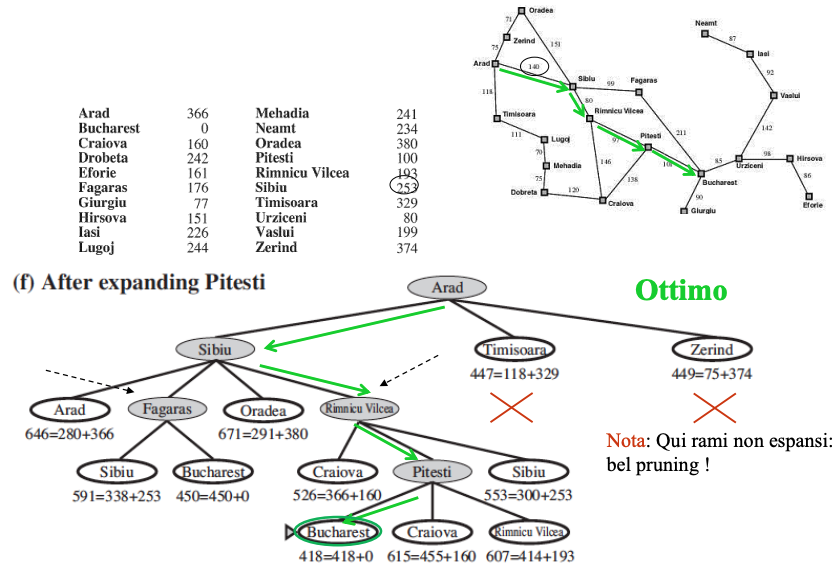
\includegraphics[width=0.62\textwidth]{images/itinerario-A*-albero.png}
    \end{figure}
\end{example}
\begin{observation}
    Alcune osservazioni su $A^*$
    \begin{enumerate}
        \item Rispetto a greedy best-first, la componente g fa si che si abbandonino cammini che vanno troppo in profondità.
        \item Ha sotto o sovra stima?
        \begin{enumerate}
            \item Una sottostima (h) può farci compiere del lavoro inutile (tenendo anche candidati non buoni), però non ci 
            fa perdere il cammino migliore (quando prendo nodo goal è il cammino migliore).
            \item Una funzione che qualche volta sovrastima può farci perdere la soluzione ottimale (taglio per causa di sovrastima, invece era buona)
        \end{enumerate}
    \end{enumerate}
\end{observation}

\subsubsection{Ottimalità su $A^*$}
Nel caso di ricerca a/su albero l'uso di un'euristica ammissibile è sufficente a garantire l'ottimalità su $A^*$.
Nel caso di ricerca su grafo (con UC come visto) serve una proprietà più forte: la \textbf{consistenza} (detta anche \textbf{monotonicità}).\\\\
Per evitare rischio di scartare candidati ottimi (stato già incontrato) ai vuol evitare, causa uso della lista esplorati, di far sparire, o meglio
non considerare al momento dell'espansione, candidati ottimali. Cerchiamo quindi condizioni per garantire che il ptimo espanso sia il migliore.
\begin{definition} 
    Un euristica \textbf{consistente} $[h(goal) = 0]$ (consistenza locale).
    $$\forall n \:\: t.c. \:\: h(n) \leq c(n, a, n') + h(n') \text{ dove n' è un successore di n}$$
\end{definition}
\hspace{-15pt}Ne segue che $f(n) \leq f(n')$
\begin{note}
    Se h è consistente la $f$ non decresce mai lungo i cammini, da cui il termine \textbf{monotona}.
\end{note}
\begin{theorem}
    Un'euristica monotona è ammissibile.
\end{theorem}
\hspace{-15pt}Esistono euristiche ammissibili che non sono monotone, ma sono rare. Le euristiche monotone garantiscino che la soluzione meno costosa 
venga trovata per rima e quindi sono ottimali anche nel caso di ricerca su grafo.\\
Non si devono recuperare tra gli antenati nodi con costo minore. Lista degli esplorati, stato già esplorato è sul cammino ottimo allora posso
evitare di inserire il corrente ripetuto senza perdere l'ottimalità.
\begin{lstlisting}
    if figlio.Stato non e in esplorati e non e in frontiera then
        frontiera = Inserisci(figlio, frontiera)
\end{lstlisting}
Per la frontiera, volendo evitare stati ripetuti, resta 'if' finale di UC:
\begin{lstlisting}
    if figlio.Stato e in frontiera con Costo-cammino piu alto then
        sostituisci quel nodo frontiera con figlio 
\end{lstlisting}